\documentclass[b5paper,10pt,twoside]{book}
\usepackage[T1]{fontenc}
\usepackage[utf8]{inputenc}
\usepackage[spanish]{babel}
\usepackage[super]{nth}
\usepackage{
    amsmath,
    amsfonts,
    amssymb,
    amsthm,
    imakeidx,
    graphicx,
    polynom,
    % subcaption,
    lipsum,
    lmodern,
    systeme,
    float,
    ifthen,
    mathrsfs,
    units,
    % enumerate,
    enumitem,
    multicol,
    geometry,
    mdframed,
    setspace,
    subcaption,
    anyfontsize,
    mathtools,
    fancyhdr,
    booktabs,
    multirow,
    csquotes,
    microtype,
    bookmark,
    emptypage,
    blkarray,
    aliascnt,
    dsfont,
    comment,
    tabularx,
    % mathds,
    titlesec,
    cancel,
    currfile,
    xcolor,
}
\usepackage[perpage]{footmisc}

\setenumerate{topsep=0pt}

\setlength{\parskip}{0.5\baselineskip}%

% \fontseries{b}\selectfont
% \renewcommand{\bfdefault}{b}

\titleformat{\chapter}
  {\normalfont\Huge}{\Huge\thechapter}{15pt}{\Huge}

% \titleformat{\section}
%   {\normalfont\large}{\large\thechapter}{15pt}{\large}

% \titleformat{\section}
%   {\normalfont\Huge}{\Huge\thechapter}{15pt}{\Huge}

% \onehalfspacing
\setstretch{1.05}
\geometry{
    margin=1in,
    % headheight=50pt,
    % headsep=12pt,
    % showframe
    % textwidth=5in,
}
% \decimalpoint
\raggedbottom
\pagestyle{plain}
% \fancyhf{}
% % \fancyheadoffset{1.0mm}
% \lhead{\includegraphics[width=0.35\textwidth]{logoECMC.png}}
% \rhead{\includegraphics[width=0.25\textwidth]{logoYachay.png}}
\fancyfoot[RO,LE]{\thepage}

\usepackage[delims=\lbrack\rbrack]{spalign}
\let\matrix=\spalignmat
\let\Amatrix=\spalignaugmat
\let\AAmatrix=\spalignaugmatn
\newcommand{\Dmatrix}[1]{\spaligndelims\vert\vert\spalignmat{#1}}

% \fancyhead[RE]{\scshape{\nouppercase{\leftmark}}}
% \fancyhead[LO]{\scshape{\nouppercase{\rightmark}}}
\renewcommand{\headrulewidth}{0pt}
\graphicspath{{images/}}
\bookmarksetup{numbered}
\makeatletter
 \renewcommand\Hy@numberline[1]{#1. }
\makeatother
\usepackage{hyperref}
\hypersetup{%
    colorlinks = {true},
            linkcolor = {blue},
            urlcolor  = {blue},
            citecolor = {blue},
            anchorcolor = {blue},
    pdftitle    ={},
    pdfauthor   ={K. Christian Chávez},
    pdfsubject  ={Abstract Algebra},
    pdfcreator  ={LaTeX},
    pdfproducer ={},
    % pdfkeywords={}{}{},
    % hidelinks,
    pdfpagemode={UseNone},
}
\newcolumntype{Y}{>{\centering\arraybackslash}X}
\renewcommand\tabularxcolumn[1]{m{#1}}
% \renewcommand\arraystretch{1.5}

\newcommand{\p}{\cdot}
\newenvironment{solution}{\noindent\textbf{\textsl{Solution}.}}{\hfill$\square$}
% \newenvironment{remark}{\noindent\textbf{\textsl{Remark.}}}{}
% \theoremstyle{definition}
% \newtheorem{problem}{Problem}%[chapter]

% \setlength\parindent{0pt}

% Nuevos comandos
\let\originalleft\left
\let\originalright\right
% \renewcommand{\left}{\mathopen{}\mathclose\bgroup\originalleft}
% \renewcommand{\right}{\aftergroup\egroup\originalright}
\newcommand{\N}{\mathds{N}}
\newcommand{\Z}{\mathds{Z}}
\newcommand{\R}{\mathds{R}}
\newcommand{\Q}{\mathds{Q}}
\newcommand{\II}{\mathds{I}}
\newcommand{\K}{\mathds{K}}
\newcommand{\PP}{\mathds{P}}
\newcommand{\C}{\mathds{C}}
\newcommand{\T}{\mathscr{T}}
\newcommand{\I}{\mathcal{I}}
\newcommand{\E}{\mathscr{E}}
\newcommand{\B}{\mathcal{B}}
\newcommand{\F}{\mathscr{F}}
\newcommand{\U}{\mathscr{U}}
\newcommand{\LL}{\mathscr{L}}
\newcommand{\OO}{\mathscr{O}}
\newcommand{\Fam}{\mathscr{F}}
\newcommand{\Nei}{\mathscr{N}}
\newcommand{\Pt}{\mathscr{P}}
% \newcommand{\ES}{\text{\upshape\O}}
% \renewcommand{\ES}{\cancel{\mathrm{O}}}
\newcommand{\ES}{\varnothing}
\newcommand{\TopS}{\left( X, \T \right)}
\newcommand{\bcap}{\bigcap}
\newcommand{\bcup}{\bigcup}
\newcommand{\dif}{\backslash}
\newcommand{\Solution}{\noindent\textbf{Solution.}}
% \let\oldbigcup\bigcup
% \renewcommand{\bigcup}{\boldsymbol{\oldbigcup}} 

\newcommand{\ev}{\textsc{ev}}
\newcommand{\ii}{\hat{\imath}}
\newcommand{\jj}{\hat{\jmath}}
\newcommand{\kk}{\hat{k}}
\newcommand{\vv}{\mathbf{v}}
\newcommand{\va}{\mathbf{a}}
\newcommand{\vb}{\mathbf{b}}
\newcommand{\vd}{\mathbf{d}}
\newcommand{\vx}{\mathbf{x}}
\newcommand{\vy}{\mathbf{y}}
\newcommand{\vu}{\mathbf{u}}
\newcommand{\vzr}{\mathbf{0}}
\newcommand{\pp}{\boldsymbol{\cdot}}
\newcommand{\AND}{\quad\text{and}\quad}
\newcommand{\seq}{\subseteq}
\newcommand{\sep}{\supseteq}
\newcommand{\nseq}{\nsubseteq}
\newcommand{\then}{\implies}
\newcommand{\abs}[1]{\left|#1\right|}
\newcommand{\Abs}[1]{\left|\!\left|#1\right|\!\right|}
\newcommand{\prt}[1]{\left(#1\right)}
\newcommand{\End}{\hfill\(\square\)}
\newcommand{\Mod}[1]{\ \left(\mathrm{mod}\ #1\right)}
\newcommand{\floor}[1]{\left\lfloor #1 \right\rfloor}
\newcommand{\ceil}[1]{\left\lceil #1 \right\rceil}
\renewcommand\labelitemi{$\bullet$}
\newcommand{\interior}[1]{#1^\circ}
\renewcommand\labelitemi{$\bullet$}
\renewcommand{\labelitemii}{$ \circ $}
\renewcommand{\mathbb}[1]{\mathds{#1}}
\renewcommand*{\thefootnote}{\fnsymbol{footnote}}

\DeclareMathOperator{\lcm}{lcm}
\DeclareMathOperator{\adj}{adj}
\DeclareMathOperator{\sen}{sen}
\DeclareMathOperator{\proy}{proy}
\DeclareMathOperator{\tr}{tr}
\DeclareMathOperator{\spn}{span}
\DeclareMathOperator{\im}{Im}
\DeclareMathOperator{\dd}{d }
\DeclareMathOperator{\card}{card}
\DeclareMathOperator{\ddd}{d\!}
% \DeclareMathOperator{\y}{y}
\DeclareMathOperator{\rank}{rank}
\DeclareMathOperator{\nul}{nul}
\DeclareMathOperator{\Int}{int}
\DeclareMathOperator{\cla}{cla}

% Añadidos después
\newcommand{\vect}[1]{\left( {#1}_{1},\dots,{#1}_{n} \right)}

\usepackage{amsthm}
\newtheoremstyle{uptheorem} 
{0.75cm}{0.75cm}{\upshape}{}{\bfseries}{.}{ }{} 
\newtheoremstyle{sltheorem} 
{0.75cm}{0.3cm}{\slshape}{}{\bfseries}{.}{ }{} 
% \theoremstyle{sltheorem}
\theoremstyle{uptheorem}
\newtheorem{theorem}{Problema}%[chapter]
\newtheorem{definition}{Definition}%[chapter]
\newcommand{\definitionautorefname}{Definition}
\newtheorem{lemma}{Lemma}%[theorem]
\newcommand{\lemmaautorefname}{Lemma}
\newtheorem{corollary}{Corollary}%[theorem]
\newcommand{\corollaryautorefname}{Corollary}
\newtheorem{corolario}{Corolario}[theorem]
\newcommand{\corolarioautorefname}{Corolario}
\theoremstyle{uptheorem} 
\newtheorem{example}{Example}%[chapter]
  \newaliascnt{examples}{example}
  \newtheorem{examples}[examples]{Examples}
  \aliascntresetthe{examples}
  \def\exampleautorefname{Example}
  \def\examplesautorefname{Examples}

\newcommand{\notaautorefname}{Nota}

\newtheoremstyle{uptheoremv2}{0.7cm}{}{\upshape}{}{\bfseries}{.}{ }{} 
\theoremstyle{uptheoremv2} 
\newtheorem{problem}[theorem]{Problema}
\newcommand{\problemautorefname}{Problem}
\newtheoremstyle{uptheoremv3}{}{}{\upshape\small}{}{\bfseries}{.}{ }{} 
\theoremstyle{uptheoremv3}
\newtheorem{remark}{Remark}[chapter]

\numberwithin{figure}{section}
\numberwithin{table}{section}
% \numberwithin{equation}{chapter}

% \usepackage[backend=biber]{biblatex}
% \bibliography{bib.bib}
% \nocite{*}

\color{black!85}

\begin{document}
\def\thetitle{Examen final}
\def\fechaentrega{31 de enero de 2025}


% \pagebreak
% \vspace*{-1.5cm}
% \begin{center}
%     
\includegraphics[height=0.075\textheight]{images/LogoClubMate.pdf} 
%         % \hspace{1cm}
%     %     \hfill
%     % 
\includegraphics[height=0.075\textheight]{images/LogoECMC.pdf}
% \end{center}

% \phantomsection\pdfbookmark{\currfilebase}{\currfilebase}

% \begin{center}
%     {\LARGE
%     Topología \\ Curso Vacacional Enero 2025\\
%     % Teaching Assistant
%     \vspace{0.5cm}
%     \textbf{\thetitle{}}}

%     % \emph{I hear, I forget;
%     % I see, I remember;
%     % I do, I understand.}
    
%     Christian Chávez\\
%     \today
% \end{center}

% % \setcounter{problem}{0}


%=================================

\begin{center}
\begin{minipage}{0.45\textwidth}
    
\includegraphics[height=0.075\textheight]{images/LogoClubMate.pdf}
\end{minipage}%
\hfill
\begin{minipage}{0.5\textwidth}
    \begin{flushright}
        {\LARGE Topología} \\ Curso Vacacional -- Enero 2025 \\
        Instructor: Christian Chávez \\
    \end{flushright}
\end{minipage}

\vspace{\baselineskip}
{\huge\thetitle} \\
% \vspace{0.5cm}

\today\\
Fecha de entrega: \fechaentrega{}

\end{center}


Todos los problemas tienen el mismo valor.
Se deben resolver exactamente \(10\) problemas
y se debe seleccionar  al menos un problema de cada sección.


% \section*{Parte 1}

\subsection*{1.\enspace Espacios Topológicos}
\addcontentsline{toc}{section}{1. Espacios Topológicos}

\begin{problem}
Sea \(X\) un conjunto.
Sea \(\mathcal{T}\) un subconjunto del conjunto potencia de \(X\).
Muestra que \(\mathcal{T}\) es una topología sobre \(X\) si, y solamente si,
\begin{enumerate}[label=(\roman*)]
\item \(\varnothing, X\in \mathcal{T}\),
\item la intersección de cualquier familia arbitraria de conjuntos cerrados de \(X\) (respecto a \(\mathcal{T}\)) es un subconjunto cerrado de \(X\) (respecto a \(\mathcal{T}\)), y 
\item la unión de cualquier familia finita de subconjuntos cerrados de \(X\) (respecto a \(\mathcal{T}\)) es un subconjunto cerrado de \(X\) (respecto a \(\mathcal{T}\)).
\end{enumerate}
\end{problem}


\begin{problem}
Considera 
\[
\Upsilon  = \left\{ 
    A\subset \Z^+ \;\bigg|\; \forall m \in \Z^+, \forall n \in A :  m|n \implies m \in A
 \right\}
\]
Muestra que \( \Omega = \left\{ O \subset \Z^+ \mid \Z^+\setminus O \in \Upsilon \right\}  \) es una topología sobre los enteros positivos.
(La relación \(\mid\) se define así:  \(a\mid b\) ssi \(ak = n\) para algún   \(k\in \Z^+\).)
\end{problem}

\begin{problem}
Considera  la colección 
\[
\mathcal{B} = \left\{ 
    [a,b) \mid a,b\in\R
 \right\}.
\]
\begin{enumerate}[label=(\roman*)]
\item Prueba  que \(\mathcal{B}\) es una base para alguna topología en \(\R\). ¿Por que esa topología es única? Esta topología se llama la topología
del límite inferior,
y el espacio topológico asociado se llama 
la línea de Sorgenfrey.


\item Muestra que la  topología
del límite inferior es más fina que la topología usual de \(\R\).

\item Muestra que en esta topología, todo abierto también es cerrado.
\end{enumerate}





\end{problem}

\subsection*{2.\enspace Espacios Métricos}
\addcontentsline{toc}{section}{2. Espacios Métricos}


\begin{problem}
Sea \(X=\mathcal{C}([0,1])\), el conjunto de todas las funciones continuas \([0,1]\to \R\).
Muestra que las
siguiente reglas de asignación 
definen métricas sobre \(X\):
\[
(f,g) \mapsto \int_0^1 |f(x) - g(x)|\mathrm{d}x
\quad\text{y}\quad
(f,g) \mapsto \sup_{x\in[0,1]} |f(x) - g(x)|.
\]

\end{problem}
 

\begin{problem}
Un espacio normado es un par \((V, \Vert \cdot \Vert)\) donde \(V\) es un espacio vectorial y \(\Vert \cdot \Vert\) es una norma sobre \(V\).
Muestra que un espacio normado se puede dotar de una topología de una manera canónica.
\end{problem}


\begin{problem}
Sea $d$ una métrica en un conjunto $X$.
Demuestra que
\begin{enumerate}[label=(\roman*)]
\item la función ${\xi} : X \times X \to [0, +\infty)$ definida por 
\[
(x, y) \mapsto \frac{d(x, y)}{1 + d(x, y)}
\]
es una métrica en $X$

\item \(\xi\) es \textbf{topológicamente equivalente} a \(d\).
\end{enumerate}
\end{problem}

\subsection*{3.\enspace Posición de un Punto Respecto  a un Conjunto}
\addcontentsline{toc}{section}{3. Posición de un Punto Respecto  a un Conjunto}


\begin{problem}
Sea \(X\) un espacio topológico y \(A\subset X\).
\begin{enumerate}[label=(\roman*)]
\item Define la clausura de \(A\) en \(X\). ¿Por qué \(\overline{A}\) es cerrado?
\item Define el interior  de \(A\) en \(X\).  ¿Por qué \({A}^\circ \) es abierto?
\end{enumerate}
\end{problem}

\begin{problem}
Sea \(A\) un subconjunto de un espacio topológico.
Demuestra que 
\begin{enumerate}[label=(\roman*)]
\item \(A\) es abierto si y solo si \(A = A^\circ\)
\item \(A\) es cerrado si y solo si \(A = \overline{A}\)
\item \(\overline{A} = A \cup A'\)
\item \(\partial A = \overline{A}\,\setminus A^\circ \)
\end{enumerate}
\end{problem}

\begin{problem}
Sea \((M,d)\) un espacio métrico,
\(A\subset X\) y \(p\in M\).
La distancia de \(p\) a \(A\)
se define como 
\[
d(p,A) = \inf\left\{ d(p,a)\mid a\in A \right\}.
\]
Supón que \(A\) es cerrado.
Prueba que \(d(p,A) = 0\) si, y solo si, \(p\in A\).
\end{problem}


\subsection*{4.\enspace Continuidad \& Homeomorfismos}
\addcontentsline{toc}{section}{4. Continuidad \& Homeomorfismos}


\begin{problem}
Sean \(X\) y \(Y\) espacios topológicos, y 
sea \(\mathcal{B}\)  una base para la topología de \(Y\).
Considera una función \(f\colon X\to Y\).
Demuestra que \(f\)
es continua si y solo si \(f^{-1}(B)\) es abierto en \(X\) para todo \(B\in \mathcal{B}\).
\end{problem}


\begin{problem}
Sea $X = \{a, b, c, d\}$ dotado de la topología
\[
\mathcal{T} = \{\varnothing, X, \{a\}, \{b\}, \{a, c\}, \{a, b\}, \{a, b, c\}\}.
\]
Define una función continua \(X\xrightarrow{\varphi} X\).
Define un homeomorfismo \(X\xrightarrow{\phi} X\) distinto de la identidad.
\end{problem}


\begin{problem}
Sea \(X\) un conjunto y 
\((Y,\mathcal{T}_Y)\) un espacio topológico.
Toma una función \(f\colon X\to Y\).
Demuestra que 
\[
\mathcal{T}_X = \left\{ 
    f^{-1}(O) \mid O\in \mathcal{T}_Y
 \right\}
\]
es una topología sobre \(X\).
Si \(X\) se dota de esta topología,
¿por qué \(f\) es continua?
\end{problem}




% \section*{Parte 2}




\subsection*{5.\enspace Propiedades Topológicas}
\addcontentsline{toc}{section}{5. Propiedades Topológicas}



\begin{problem}
Sea \(X\)  un espacio topológico.
\begin{enumerate}[label=(\roman*)]
\item Define densidad respecto al espacio y respecto a un super conjunto (\(B\) es super conjunto de \(A\) si \(B\) contiene a \(A\), i.e. \(B\supset A\)).
\item Sea   \(D\subset X\). Muestra que \(\overline{D} = X\) si, y solamente si, \(D\) interseca a todo abierto no vacío de \(X\).
\end{enumerate}



\end{problem}

\begin{problem}
Sea \(f\colon X\to Y\)
un homeomorfismo.
Recuerda que una propiedad topológica es aquella que se puede enunciar en términos de 
conjuntos abiertos.
Una invariante topológica 
es una propiedad que se preserva bajo homeomorfismos.
Demuestra que 
\begin{enumerate}[label=(\roman*)]
\item  \(X\) es Hausdorff si y solamente si  \(Y\) lo es,
\item  \(X\) es conexo si y solamente si  \(Y\) lo es,
\item  \(X\) es conexo por caminos si y solamente si  \(Y\) lo es,
\item  \(X\) es compacto si y solamente si  \(Y\) lo es,
\end{enumerate}
\end{problem}

\pagebreak

\begin{problem}\hfill
\begin{enumerate}[label=(\roman*)]
\item Define  el segundo  axioma de numerabilidad  {\scshape anii}.
\item Define segundo  axioma de separación \(\mathbf{T}_2\).
\item Prueba que un espacio métrico es  Hausdorff.
\item Prueba que si un espacio métrico es segundo contable, entonces es separable. (Recuerda: un espacio topológico es separable si contiene un subconjunto que es denso en todas partes y que es contable.)
\end{enumerate}

\end{problem}


\subsection*{6.\enspace Construcciones Topológicas}
\addcontentsline{toc}{section}{6. Construcciones Topológicas}


\begin{problem}
Sea \((X_\lambda, \mathcal{T}_\Lambda)_{\lambda\in\Lambda}\)
una familia finita de espacios topológicos.
\begin{enumerate}[label=(\roman*)]
\item Define 
la topología producto sobre \(\prod\limits_{\lambda\in\Lambda} X_\lambda\).

\item Define las proyecciones canónicas y muestra que son continuas respecto a la topología producto. ¿Qué significa que la topología producto sea la más gruesa (= débil) para la cual las proyecciones canónicas son continuas?
\end{enumerate}

\end{problem}

 
\begin{problem}
Sea \(X\times Y\) dotado de la topología 
producto.
\begin{enumerate}[label=(\roman*)]
\item Describe los entornos  de un punto  \(p\in X\times Y\).
\item Demuestra que si \(X\) y \(Y\) son Hausdorff, \(X\times Y\) también.
\end{enumerate}

\end{problem}

\begin{problem}\hfill\null
\begin{enumerate}[label=(\roman*)]
\item Define qué es una relación de equivalencia.
\item Muestra que una relación de equivalencia induce una partición de manera canónica y vice versa.
% \item Muestra que una partición induce una relación de equivalencia de manera canónica,
\item El conjunto cociente de un conjunto \(X\) por una relación de equivalencia \(\sim\) (sobre \(X\)) se denota \(X/\!\!\sim\). Da la definición precisa de \(X/\!\!\sim\).
\item Define la proyección canónica \(\pi\colon X\to X/\!\!\sim\)
\end{enumerate}
\end{problem}


\begin{problem}
Sea \((X,\mathcal{T})\) 
un espacio topológico
y \(\sim\) una relación 
de equivalencia sobre
\(X\).
Demuestra 
que la colección
\[
\mathcal{Q} = \left\{ 
    A\subset X/\!\!\sim \;\bigg|\; \pi^{-1}(A)\in  \mathcal{T}
 \right\}
\]
es una topología
en \(X/\!\!\sim\).
\end{problem}

\pagebreak

\begin{problem}
El toro topológico se define como el espacio  producto   \(S^1\times S^1\).
Sabemos que 
\[
S^1\times S^1 \cong I^2 / [(0,t)\sim(1,t),\; (t,0)\sim (t,1)].
\]
\begin{figure}[!htb]
    \centering
    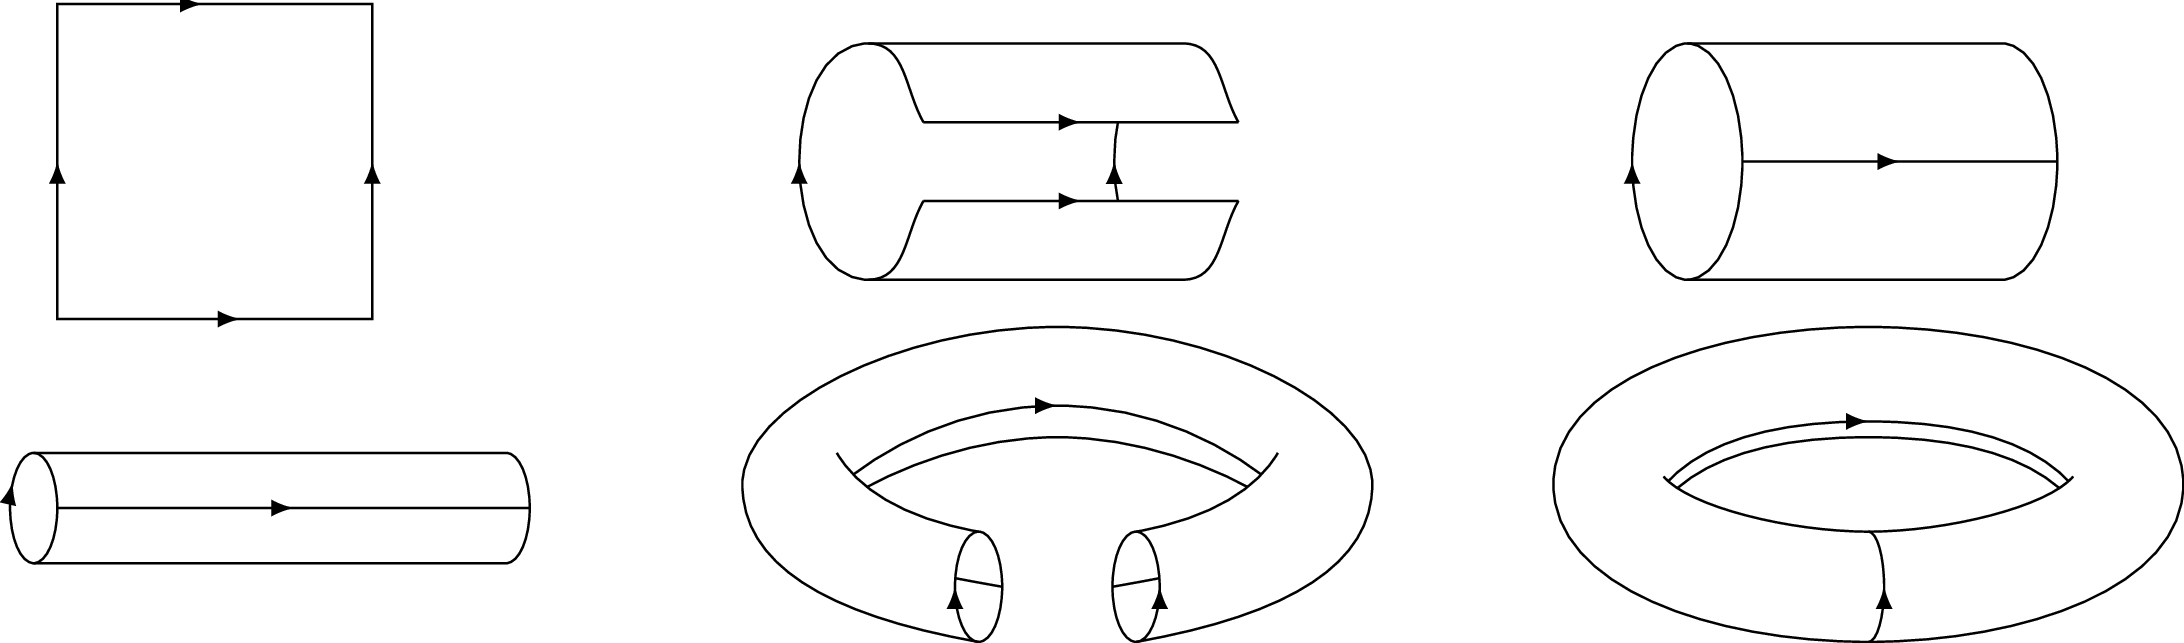
\includegraphics[width=0.85\textwidth]{plane-to-torus.png}
    % \caption{El t}%\label{fig:}
\end{figure}


Describe explícitamente \(\sim\) y la partición que ella genera.
Aquí \(I\) denota el 
intervalo unitario \([0,1]\).
\end{problem}

\end{document}

